\documentclass[11pt,a4paper]{article}
\usepackage[utf8]{inputenc}
\usepackage[T1]{fontenc}
\usepackage{fouriernc}
\usepackage{tikz}
\usetikzlibrary{arrows.meta}
\usepackage[french]{babel}
\frenchbsetup{StandardLists=true}
\NoAutoSpaceBeforeFDP
\usepackage{enumitem}
\usepackage{amsmath}
\usepackage{amssymb}
\usepackage[left=2cm,right=2cm,top=2cm,bottom=2cm]{geometry}
\usepackage[dvipsnames]{xcolor}
\usepackage{graphicx}
\usepackage{setspace}
\singlespacing
\usepackage{tcolorbox}
\usepackage{multicol}
\usepackage{multirow}
\usepackage{tabularx}
\usepackage{booktabs}
\usepackage{pifont}
\usepackage{array}
\usepackage{fancyhdr}
\setlength{\headheight}{14pt}

\pagestyle{fancy}
\renewcommand\headrulewidth{1pt}
\fancyhead[L]{Lycée Denis Diderot}
\fancyhead[R]{Classe : T~Micro}
\setcounter{page}{1}
\fancyfoot[C]{Les moteurs --- Devoir --- page~\thepage}
\fancyfoot[R]{\today}
\fancyfoot[L]{Alexis RUIZ}

\setlength{\parindent}{0pt}
\renewcommand{\arraystretch}{1.8}

\newcommand{\cadreblanc}[1]{%
	\medskip\framebox[\linewidth][c]{%
		\rule{0mm}{#1mm}}\par
	\medskip}

\newcommand*\acocher{\leavevmode{\fboxsep0pt \fboxrule0.8pt \fbox{\vrule height1.8ex depth.1ex width0pt \vrule height0pt depth0pt width1.9ex }}}

\begin{document}

\begin{center}
	\LARGE{\textbf{Les moteurs --- Devoir}}

	\vspace{3mm}

	\large{Durée : 1 heure}
\end{center}

\hrule
\vspace{2mm}

\textbf{Nom :} \dotfill \hspace{2cm} \textbf{Prénom :} \dotfill \hspace{2cm} \textbf{Date :} \dotfill

\vspace{3mm}

\begin{tcolorbox}[colback=blue!5!white, colframe=blue!75!black]
	\textbf{Consignes :}
	\begin{itemize}
		\item Répondre sur le sujet
		\item Justifier les calculs : formule, application numérique, unité
		\item Soigner la présentation et l'orthographe
		\item Le barème indicatif est donné à titre informatif
	\end{itemize}
\end{tcolorbox}

\vspace{3mm}
\hrule
\vspace{4mm}

%%%%%%%%%%%%%%%%%%%%%%%%%%%%%%%%%%%%%%%%%%
\textbf{Exercice 1 : Comment vérifier la compatibilité d'un moteur ?}
\hfill \textbf{/7 points}

\vspace{3mm}

\begin{minipage}[h]{0.60\linewidth}
	Un technicien doit remplacer le moteur d'un ascenseur.
	Les caractéristiques du moteur à remplacer sont indiquées
	sur la plaque signalétique ci-contre.
	\vspace{3mm}

	Dans son atelier, il dispose des moteurs suivants :
\end{minipage}
\hfill
\begin{minipage}[h]{0.36\linewidth}
	\begin{center}
		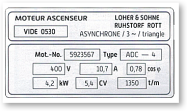
\includegraphics[width=5.8cm]{images/plaque.png}

		\textit{\small Plaque signalétique}
	\end{center}
\end{minipage}

\vspace{4mm}

\begin{center}
	\renewcommand{\arraystretch}{1.8}
	\begin{tabular}{|c|l|c|c|c|}
		\hline
		\textbf{Modèle} & \textbf{Type} & $\boldsymbol{P_{\rm utile}}$ & \textbf{Rendement} & $\boldsymbol{n}$ (tr/min) \\
		\hline
		1 & Courant continu & 4,5~kW & 0,70 & 1350 \\
		\hline
		2 & Asynchrone & 4,0~kW & 0,80 & 1350 \\
		\hline
		3 & Asynchrone & 4,1~kW & 0,80 & 1350 \\
		\hline
		4 & Asynchrone & 4,2~kW & 0,78 & 1350 \\
		\hline
	\end{tabular}
\end{center}

\vspace{5mm}

\textbf{1.} Quel type de moteur correspond à la plaque signalétique ? \hfill \textit{(0,5~pt)}

\cadreblanc{12}

\textbf{2.} Donner les différentes grandeurs physiques présentes sur cette plaque ainsi que leurs unités.
\hfill \textit{(1,5~pt)}

\cadreblanc{20}

\textbf{3.} D'après le tableau, sur quels critères le technicien doit-il choisir son moteur ?
\hfill \textit{(0,5~pt)}

\cadreblanc{14}

\textbf{4.} Calculer la puissance électrique absorbée $P_a$ par le moteur à remplacer.
\hfill \textit{Donnée : $P_a = \sqrt{3} \times U \times I \times \cos\varphi$}
\hfill \textit{(1,5~pt)}

\cadreblanc{28}

\textbf{5.} Calculer le rendement $\eta$ du moteur à remplacer.
\hfill \textit{Donnée : $\eta = \dfrac{P_{\rm utile}}{P_a}$}
\hfill \textit{(1,5~pt)}

\cadreblanc{28}

\textbf{6.} Comparer la puissance utile et le rendement du moteur à remplacer avec ceux des moteurs disponibles. Quel moteur le technicien doit-il choisir ? \hfill \textit{(1~pt)}

\cadreblanc{16}

\textbf{7.} Rédiger un court texte expliquant comment choisir le bon moteur de remplacement.
\hfill \textit{(0,5~pt)}

\cadreblanc{22}

\vfill
\newpage

%%%%%%%%%%%%%%%%%%%%%%%%%%%%%%%%%%%%%%%%%%
\textbf{Exercice 2 : QCM} \hfill \textbf{/4 points}

\vspace{2mm}

Parmi les trois propositions, choisissez la bonne réponse.

\vspace{3mm}

\begin{center}
\renewcommand{\arraystretch}{2.5}
\begin{tabular}{|m{4mm}|p{4.5cm}||m{3.5cm}|m{3.5cm}|m{3.5cm}|}
	\hline
	\ding{202} & Le moteur électrique est un convertisseur qui transforme :
		& \acocher~de l'énergie mécanique en énergie électrique
		& \acocher~de l'énergie électrique en énergie mécanique
		& \acocher~de l'énergie thermique en énergie électrique \\
	\hline
	\ding{203} & Le rendement d'un moteur est :
		& \acocher~toujours supérieur à 1
		& \acocher~toujours égal à 1
		& \acocher~toujours inférieur à 1 \\
	\hline
	\ding{204} & Pour faire varier la fréquence de rotation d'un moteur asynchrone, il faut faire varier :
		& \acocher~la résistance de l'induit
		& \acocher~la fréquence de la tension d'alimentation
		& \acocher~uniquement l'intensité du courant \\
	\hline
	\ding{205} & La fréquence de rotation d'un moteur peut s'exprimer en :
		& \acocher~Hertz (Hz)
		& \acocher~tours par minute (tr/min) ou rad/s
		& \acocher~Watts (W) \\
	\hline
	\ding{206} & La tension d'alimentation d'un moteur s'exprime en :
		& \acocher~Ampères (A)
		& \acocher~Ohms ($\Omega$)
		& \acocher~Volts (V) \\
	\hline
	\ding{207} & Sur la plaque signalétique d'un moteur, on peut lire :
		& \acocher~le prix d'achat du moteur
		& \acocher~la puissance utile, la tension et la vitesse de rotation
		& \acocher~uniquement le type de moteur \\
	\hline
	\ding{208} & La force électromotrice $E$ d'un moteur à courant continu est :
		& \acocher~indépendante de la vitesse de rotation
		& \acocher~toujours égale à la tension d'alimentation $U$
		& \acocher~proportionnelle à la vitesse de rotation $n$ \\
	\hline
\end{tabular}
\end{center}

\vfill
\newpage

%%%%%%%%%%%%%%%%%%%%%%%%%%%%%%%%%%%%%%%%%%
\textbf{Exercice 3 : Rendement d'un moteur asynchrone}
\hfill \textbf{/4 points}

\vspace{4mm}

Patrice obtient le bilan de puissance du moteur asynchrone suivant, mais les données sont incomplètes.
Il se souvient que :
\[P_e = P_m + \sum \text{pertes}\]

\vspace{4mm}

\begin{center}
\begin{tikzpicture}[>=Stealth, font=\small]

	\tikzset{
		boite/.style={draw, rounded corners=3pt, align=center,
		              text width=3cm, inner sep=4pt},
	}

	% ---- Photo du moteur au centre ----
	\node[anchor=center] (moteur) at (0,0)
		{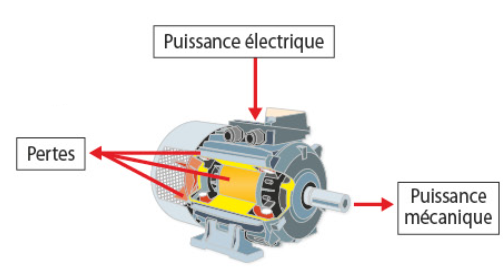
\includegraphics[width=11cm]{images/moteur_propre.png}};

	% ---- Puissance électrique (haut) ----
	\node[boite, fill=blue!8, draw=blue!60!black,
	      text width=5.4cm] (Pe) at (0, 2.2)
		{\textbf{Puissance électrique}\\[2pt]
		 \large$P_e = \boldsymbol{?}$~\textbf{kW}};
	%\draw[->, very thick, blue!70!black] (Pe.south) -- (0,2.1);

	% ---- Pertes stator (gauche haut) ----
	\node[boite, fill=orange!10, draw=orange!70!black,
	      text width=3.2cm] (Pst) at (-5.3, 0.4)
		{\textbf{Pertes stator}\\(Joule + fer)\\[2pt]
		 \large\textbf{1~745~W}};
	%\draw[->, thick, orange!70!black] (Pst.east) -- (-2.8, 1.2);

	% ---- Pertes rotor (gauche bas) ----
	\node[boite, fill=orange!10, draw=orange!70!black,
	      text width=3.2cm] (Pro) at (-5.3, -1.0)
		{\textbf{Pertes rotor}\\(Joule + fer)\\[2pt]
		 \large\textbf{855~W}};
	%\draw[->, thick, orange!70!black] (Pro.east) -- (-2.8, -0.5);

	% ---- Puissance mécanique (droite) ----
	\node[boite, fill=red!8, draw=red!60!black,
	      text width=3.4cm] (Pm) at (5, -1.50)
		{\textbf{Puissance mécanique}\\[2pt]
		 \large$P_m = \textbf{14{,}5}$~\textbf{kW}};
	%\draw[->, very thick, red!70!black] (2.8,0) -- (Pm.west);

	% ---- Pertes mécaniques (bas) ----
	\node[boite, fill=orange!10, draw=orange!70!black,
	      text width=3.2cm] (Pmec) at (-5.30, -2.9)
		{\textbf{Pertes mécaniques}\\(frottements, roulements)\\[2pt]
		 \large$\boldsymbol{?}$~\textbf{kW}};
	%\draw[->, thick, orange!70!black] (0,-2.1) -- (Pmec.north);

	% ---- Rendement (cercle haut droit) ----
	\draw[thick, fill=red!12, draw=red!70!black] (5.5, 3.0) circle (1.5cm);
	\node[align=center, red!80!black, font=\bfseries] at (5.5, 3.0)
		{Rendement\\\large$\eta = 81~\%$};

\end{tikzpicture}
\end{center}

\vspace{6mm}

\textbf{1.} Calculer la puissance électrique absorbée $P_e$ par le moteur. \hfill \textit{(2~pts)}

\cadreblanc{40}

\textbf{2.} Calculer les pertes mécaniques du moteur. \hfill \textit{(2~pts)}

\cadreblanc{40}

\vfill
\newpage

%%%%%%%%%%%%%%%%%%%%%%%%%%%%%%%%%%%%%%%%%%
\textbf{Exercice 4 : Fréquence de rotation et force électromotrice}
\hfill \textbf{/5 points}

\vspace{4mm}

Suite à une réparation, Gaston mesure, à vide, la tension $U$ aux bornes de l'induit d'un moteur à courant continu, l'intensité $I$ du courant absorbé par l'induit et la fréquence de rotation $n$. Un ohmmètre placé aux bornes de l'induit indique une résistance $r = 0{,}9~\Omega$.

\vspace{4mm}

\textbf{1.} Calculer la force électromotrice $E$ du moteur pour $U = 100$~V et $I = 12{,}1$~A.
\hfill \textit{Donnée : $E = U - r \cdot I$} \hfill \textit{(1~pt)}

\cadreblanc{12}

\textbf{2.} Compléter les données manquantes dans le tableau. \hfill \textit{(2~pts)}

\vspace{3mm}

\begin{center}
	\renewcommand{\arraystretch}{2.2}
	\begin{tabular}{|l|c|c|c|c|c|}
		\hline
		$U$ (en~V) & 100 & 161 & 242 & 324 & 407 \\
		\hline
		$I$ (en~A) & 12,1 & & 34 & 44,1 & 51,8 \\
		\hline
		$n$ (en~tr/min) & 500 & & & & \\
		\hline
		$E$ (en~V) & & 140 & & & 361 \\
		\hline
	\end{tabular}
\end{center}

\vspace{4mm}

\textbf{3.} Placer les points de coordonnées $(n\,;\,E)$ dans le repère orthogonal ci-dessous.
\hfill \textit{(1,5~pt)}

\vspace{4mm}

\begin{center}
\begin{tikzpicture}[scale=1]
	% Fine grid
	\draw[very thin, gray!30] (0,0) grid[xstep=0.2, ystep=0.2] (10,7);
	% Main grid
	\draw[thin, gray!60] (0,0) grid[xstep=2, ystep=1] (10,7);
	% Axes
	\draw[->, thick] (0,0) -- (10.4,0) node[right] {$n$ (tr/min)};
	\draw[->, thick] (0,0) -- (0,7.4) node[above] {$E$ (en~V)};
	% X axis ticks and labels (2cm = 500 tr/min)
	\foreach \x/\lbl in {2/500, 4/1000, 6/1500, 8/2000, 10/2500}{
		\draw[thick] (\x, 0.08) -- (\x, -0.08);
		\node[below, font=\small] at (\x, 0) {\lbl};
	}
	% Y axis ticks and labels (1cm = 50 V)
	\foreach \y/\lbl in {1/50, 2/100, 3/150, 4/200, 5/250, 6/300, 7/350}{
		\draw[thick] (0.08, \y) -- (-0.08, \y);
		\node[left, font=\small] at (0, \y) {\lbl};
	}
	% Origin label
	\node[below left, font=\small] at (0,0) {0};
\end{tikzpicture}
\end{center}

\vspace{3mm}

\textbf{4.} Que peut-on constater sur ce graphique ? Que peut-on conclure concernant la relation entre $E$ et $n$ ? \hfill \textit{(0,5~pt)}

\cadreblanc{22}

\vfill


\end{document}
